
\begin{figure}
\resizebox{0.28\textheight}{!}{
\begin{subfigure}{.5\linewidth}
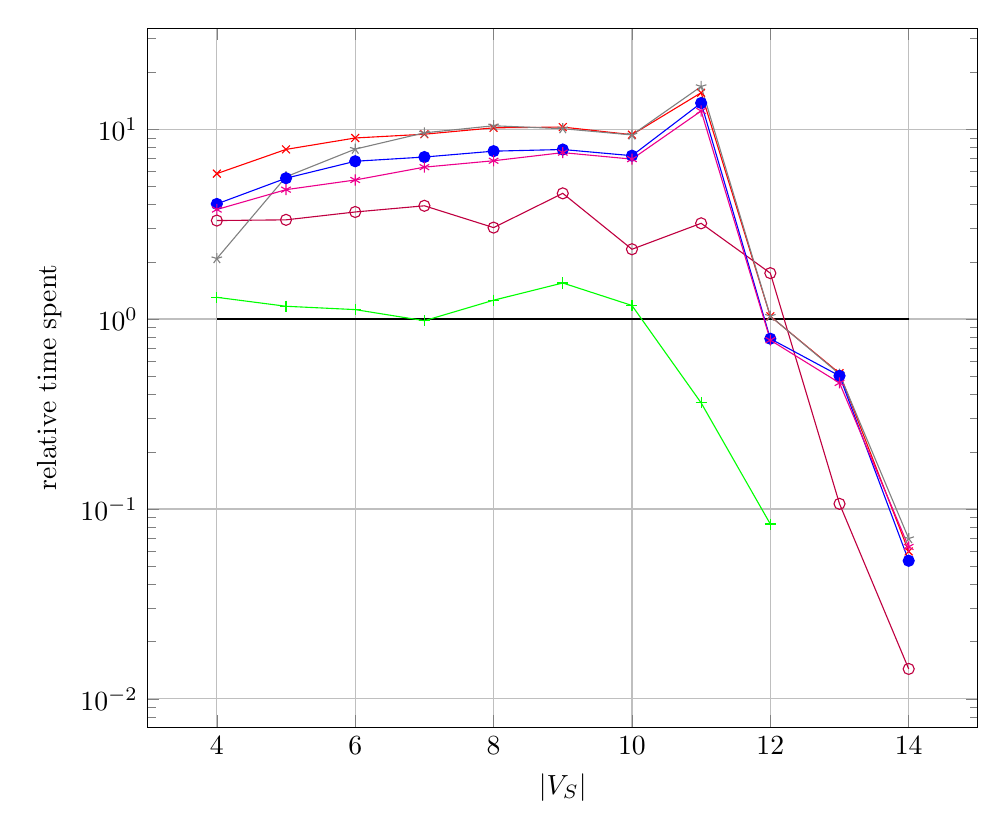
\begin{tikzpicture}
    \begin{axis}[
        xlabel=$|V_S|$,
        ylabel=relative time spent,
        ymode=log,
        legend style={at={(0.9,0.1)},anchor=south east},
        width=\textwidth,
		y tick label style={/pgf/number format/sci},
        ymajorgrids,
        xmajorgrids,		
    ]
\addplot [mark=none, black] plot coordinates {
        (4,1) (14,1)};




\addplot[
        mark=x,
        red,
    ] plot coordinates {
        (4,5.829952304363644)
        (5,7.821514135009583)
        (6,8.982363969917358)
        (7,9.401332680691212)
        (8,10.158832279951605)
        (9,10.252325251025706)
        (10,9.34581888789391)
        (11,15.546748123060839)
        (12,1.0341526662898237)
        (13,0.5183898969146863)
        (14,0.05971709064829511)
};
%    \addlegendentry{DFS}


\addplot[
        mark=o,
        purple,
    ] plot coordinates {
        (4,3.3007473913750918)
        (5,3.3292641262270837)
        (6,3.6622616535723047)
        (7,3.9481137630108396)
        (8,3.030286162147374)
        (9,4.590014716545663)
        (10,2.330905974473567)
        (11,3.192281658331693)
        (12,1.744595348175264)
        (13,0.10640200382876541)
        (14,0.014374937918376296)
};
%    \addlegendentry{GDFS O IP}


\addplot[
        mark=star,
        gray,
    ] plot coordinates {
        (4,2.081240181067252)
        (5,5.613910854682754)
        (6,7.849457219522296)
        (7,9.56049923079753)
        (8,10.416398040783026)
        (9,10.0534722450281)
        (10,9.318833737054117)
        (11,16.77294360448037)
        (12,1.036148432755423)
        (13,0.5131767288245823)
        (14,0.06986347139547233)
};
%    \addlegendentry{GDFS C}


\addplot[
        mark=*,
        blue,
    ] plot coordinates {
        (4,4.036935610516745)
        (5,5.515429351367027)
        (6,6.774063252800069)
        (7,7.129623094348765)
        (8,7.656237850184846)
        (9,7.811733342175969)
        (10,7.246802908944303)
        (11,13.722983859104243)
        (12,0.7878416162899551)
        (13,0.502222694200184)
        (14,0.053345329755408066)
};
%    \addlegendentry{K-Path}
\addplot[
        mark=+,
        green,
    ] plot coordinates {
        (4,1.3011349314115381)
        (5,1.1674190431355977)
        (6,1.1211917642297184)
        (7,0.9799097022873059)
        (8,1.2563225326740295)
        (9,1.5481480597546917)
        (10,1.17848246411115)
        (11,0.3618711611946529)
        (12,0.08327602042560134)
};
%    \addlegendentry{CP}


\addplot[
        mark=asterisk,
        magenta,
    ] plot coordinates {
        (4,3.7736038154304787)
        (5,4.800389319350771)
        (6,5.397341566198895)
        (7,6.306734163350917)
        (8,6.815885755656629)
        (9,7.520888523608972)
        (10,6.951520443072349)
        (11,12.458753170545519)
        (12,0.7742934930427632)
        (13,0.46088425014379175)
        (14,0.06313695543283937)
};
%    \addlegendentry{GDFS A IP}





    \end{axis}
    \end{tikzpicture}
\caption{$|V_T|=1\frac{1}{2}*|V_S|$ (no caching)}
\end{subfigure}%
}
\resizebox{0.28\textheight}{!}{
\begin{subfigure}{.5\linewidth}
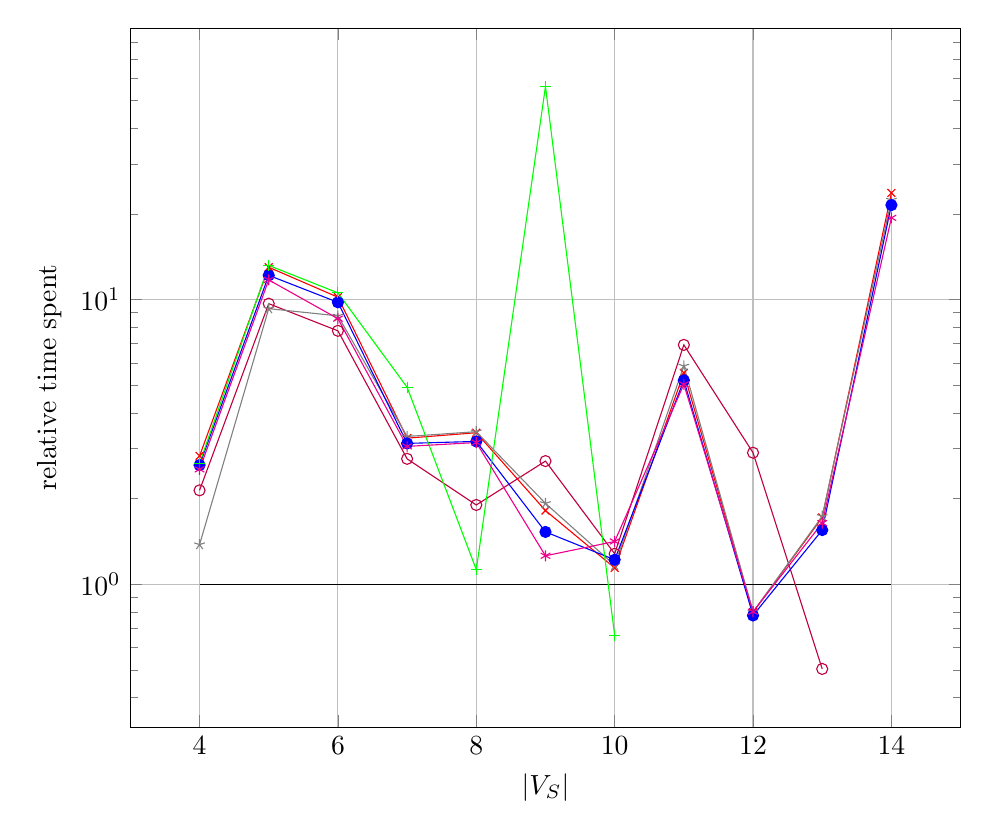
\begin{tikzpicture}
    \begin{axis}[
        xlabel=$|V_S|$,
        ylabel=relative time spent,
        ymode=log,
        legend style={at={(0.9,0.1)},anchor=south east},
        width=\textwidth,
		y tick label style={/pgf/number format/sci},
        ymajorgrids,
        xmajorgrids,		
    ]
\addplot [mark=none, black] plot coordinates {
        (4,1) (14, 1)};





\addplot[
        mark=x,
        red,
    ] plot coordinates {
        (4,2.8251795368790886)
        (5,12.999580346656751)
        (6,10.202174684933484)
        (7,3.262604211259584)
        (8,3.408918438863976)
        (9,1.8166545299203807)
        (10,1.1422160886456934)
        (11,5.530516473257274)
        (12,0.7986133987525276)
        (13,1.7180491450318693)
        (14,23.721522460227753)
};
%    \addlegendentry{DFS}
\addplot[
        mark=o,
        purple,
    ] plot coordinates {
        (4,2.1391785196119923)
        (5,9.683057001857964)
        (6,7.773825041515071)
        (7,2.7604466990768595)
        (8,1.9008757163878494)
        (9,2.7101513865191915)
        (10,1.2805148059566114)
        (11,6.937603075441524)
        (12,2.9004853202789205)
        (13,0.5045390730335063)
};
%    \addlegendentry{GDFS O IP}


\addplot[
        mark=star,
        gray,
    ] plot coordinates {
        (4,1.3794140730076914)
        (5,9.299733094390856)
        (6,8.772951593738188)
        (7,3.307376496667975)
        (8,3.4383266889141892)
        (9,1.9254251970590692)
        (10,1.1671557982423402)
        (11,5.851599859841392)
        (12,0.7997588706522294)
        (13,1.7348281924961175)
        (14,22.40100510075956)
};
%    \addlegendentry{GDFS C}


\addplot[
        mark=*,
        blue,
    ] plot coordinates {
        (4,2.6239880026319113)
        (5,12.176055240511092)
        (6,9.786244499035096)
        (7,3.127359936505137)
        (8,3.1774880567968005)
        (9,1.528458868204552)
        (10,1.2199898778953424)
        (11,5.209122239775357)
        (12,0.7776618244283469)
        (13,1.5513809856510496)
        (14,21.49466036911607)
};
%    \addlegendentry{K-Path}


\addplot[
        mark=+,
        green,
    ] plot coordinates {
        (4,2.6615145962479296)
        (5,13.192185281822104)
        (6,10.56726292801845)
        (7,4.92388122723026)
        (8,1.126596319598566)
        (9,56.0969304160683)
        (10,0.6621016861467689)
};
%    \addlegendentry{CP}


\addplot[
        mark=asterisk,
        magenta,
    ] plot coordinates {
        (4,2.5345706323293955)
        (5,11.732948804586153)
        (6,8.577253069471816)
        (7,3.052311500224188)
        (8,3.1492268511393373)
        (9,1.2598729843415928)
        (10,1.414481795839197)
        (11,5.042048634623404)
        (12,0.8013450614402682)
        (13,1.642270880020916)
        (14,19.386486921496203)
};
%    \addlegendentry{GDFS A IP}



	
    \end{axis}
    \end{tikzpicture}

\caption{$|V_T|=1\frac{1}{2}*|V_S|$ (cached)}
\end{subfigure}
}
\newline
\resizebox{0.28\textheight}{!}{
\begin{subfigure}{0.5\linewidth}

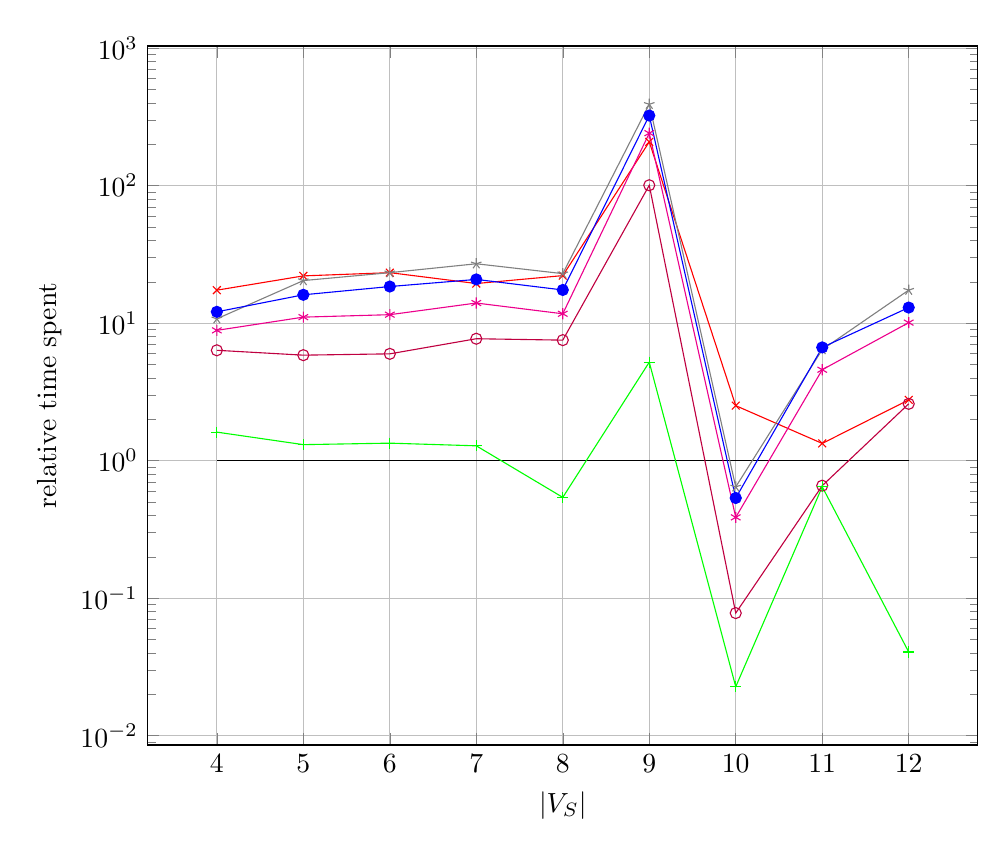
\begin{tikzpicture}
    \begin{axis}[
        xlabel=$|V_S|$,
        ylabel=relative time spent,
        ymode=log,
        legend style={at={(0.9,0.1)},anchor=south east},
        width=\textwidth,
		y tick label style={/pgf/number format/sci},
        ymajorgrids,
        xmajorgrids,		
    ]
\addplot [mark=none, black] plot coordinates {
        (4,1) (12, 1)};
        
%    \node[] at (axis cs: 9,1.1) {Awaiting test results (CAES server)};


\addplot[
        mark=x,
        red,
    ] plot coordinates {
        (4,17.386687830540524)
        (5,22.079291788970327)
        (6,23.306743149976228)
        (7,19.430501058064742)
        (8,22.18188165942091)
        (9,208.2138028355397)
        (10,2.513700580968542)
        (11,1.3354403700554096)
        (12,2.769685497589875)
};
%    \addlegendentry{DFS}


\addplot[
        mark=o,
        purple,
    ] plot coordinates {
        (4,6.352134028283731)
        (5,5.854587074510253)
        (6,5.985860240907849)
        (7,7.709398766817202)
        (8,7.530947931423977)
        (9,100.71864029454015)
        (10,0.07798933813487574)
        (11,0.6582569130981772)
        (12,2.5920862258520847)
};
%    \addlegendentry{GDFS O IP}
\addplot[
        mark=star,
        gray,
    ] plot coordinates {
        (4,10.761013649646893)
        (5,20.41574344572187)
        (6,23.304616084965065)
        (7,27.046121301467018)
        (8,22.92486770453236)
        (9,390.8923046050332)
        (10,0.6451925167117611)
        (11,6.426992380187482)
        (12,17.397334287179326)
};
%    \addlegendentry{GDFS C}


\addplot[
        mark=*,
        blue,
    ] plot coordinates {
        (4,12.096262623777024)
        (5,16.08617175919)
        (6,18.475144819368374)
        (7,20.81253092789625)
        (8,17.4435299319244)
        (9,323.5049321924643)
        (10,0.5356093481057399)
        (11,6.667174509238782)
        (12,12.992684943846735)
};
%    \addlegendentry{K-Path}


\addplot[
        mark=+,
        green,
    ] plot coordinates {
        (4,1.6139175990246586)
        (5,1.308680553430318)
        (6,1.3420234704630691)
        (7,1.2831364418331979)
        (8,0.5413740631720213)
        (9,5.2062116151636655)
        (10,0.02272540669855816)
        (11,0.646307333488348)
        (12,0.04065603348894453)
};
%    \addlegendentry{CP}


\addplot[
        mark=asterisk,
        magenta,
    ] plot coordinates {
        (4,8.870187999266555)
        (5,11.06879290067633)
        (6,11.530569519342539)
        (7,14.018534191414552)
        (8,11.707182654942214)
        (9,240.92574467452093)
        (10,0.3875006668882859)
        (11,4.588294705762263)
        (12,10.093545772616306)
};
%    \addlegendentry{GDFS A IP}


    \end{axis}
    \end{tikzpicture}

\caption{$|V_T|=3*|V_S|$ (no caching)}

\end{subfigure}
}
\resizebox{0.28\textheight}{!}{
\begin{subfigure} {0.5\linewidth}

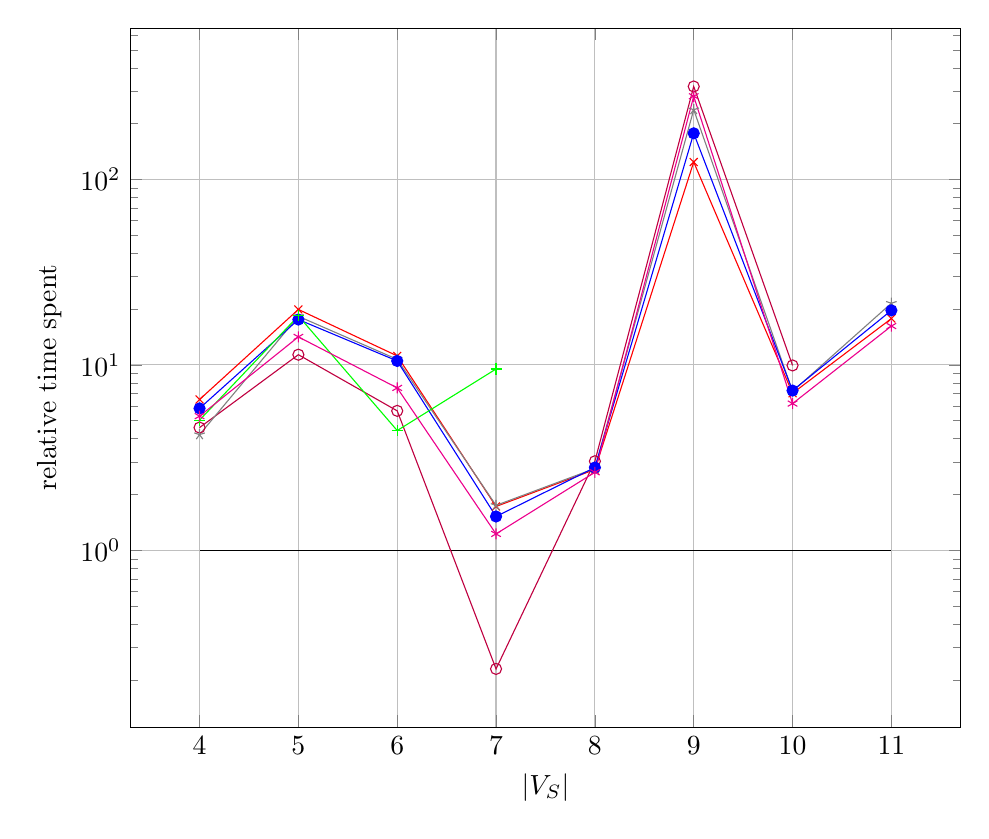
\begin{tikzpicture}
    \begin{axis}[
        xlabel=$|V_S|$,
        ylabel=relative time spent,
        ymode=log,
        legend style={at={(0.9,0.1)},anchor=south east},
        width=\textwidth,
		y tick label style={/pgf/number format/sci},
        ymajorgrids,
        xmajorgrids,		
    ]
\addplot [mark=none, black] plot coordinates {
        (4,1) (11, 1)};

%    \node[] at (axis cs: 9,1.1) {Awaiting test results (CAES server)};


\addplot[
        mark=x,
        red,
    ] plot coordinates {
        (4,6.506721650403205)
        (5,19.909363887543122)
        (6,11.177297154921606)
        (7,1.724519080351556)
        (8,2.7285266745194945)
        (9,124.16181657015836)
        (10,7.031445004959032)
        (11,17.775679517060333)
};
%    \addlegendentry{DFS}


\addplot[
        mark=o,
        purple,
    ] plot coordinates {
        (4,4.591167743768188)
        (5,11.350912752822408)
        (6,5.65138232112045)
        (7,0.22941169442122966)
        (8,3.022521866223289)
        (9,317.2200653821222)
        (10,9.933613641908536)
};
%    \addlegendentry{GDFS O IP}


\addplot[
        mark=star,
        gray,
    ] plot coordinates {
        (4,4.207074680497982)
        (5,18.284434265485746)
        (6,10.709129649746266)
        (7,1.7482843191894677)
        (8,2.7628381393187915)
        (9,237.7691906661526)
        (10,7.2060962391545695)
        (11,21.510504634766995)
};
%    \addlegendentry{GDFS C}


\addplot[
        mark=*,
        blue,
    ] plot coordinates {
        (4,5.828596980071678)
        (5,17.56552393240703)
        (6,10.500132546594331)
        (7,1.5222497146218434)
        (8,2.7964449321329083)
        (9,177.3520386845159)
        (10,7.269881235493629)
        (11,19.678511605024486)
};
%    \addlegendentry{K-Path}
\addplot[
        mark=+,
        green,
    ] plot coordinates {
        (4,5.034988757242889)
        (5,18.379644895855858)
        (6,4.42492369951899)
        (7,9.504410596005838)
};
%    \addlegendentry{CP}


\addplot[
        mark=asterisk,
        magenta,
    ] plot coordinates {
        (4,5.291688590357283)
        (5,14.16162037925404)
        (6,7.513687814173463)
        (7,1.2262338445252592)
        (8,2.635480706053349)
        (9,280.95194542270235)
        (10,6.186575229718758)
        (11,16.197435578006964)
};
%    \addlegendentry{GDFS A IP}


	
    \end{axis}
    \end{tikzpicture}
\caption{$|V_T|=3*|V_S|$ (cached)}

\end{subfigure}
}
\newline
\resizebox{0.28\textheight}{!}{
\begin{subfigure} {0.5\linewidth}

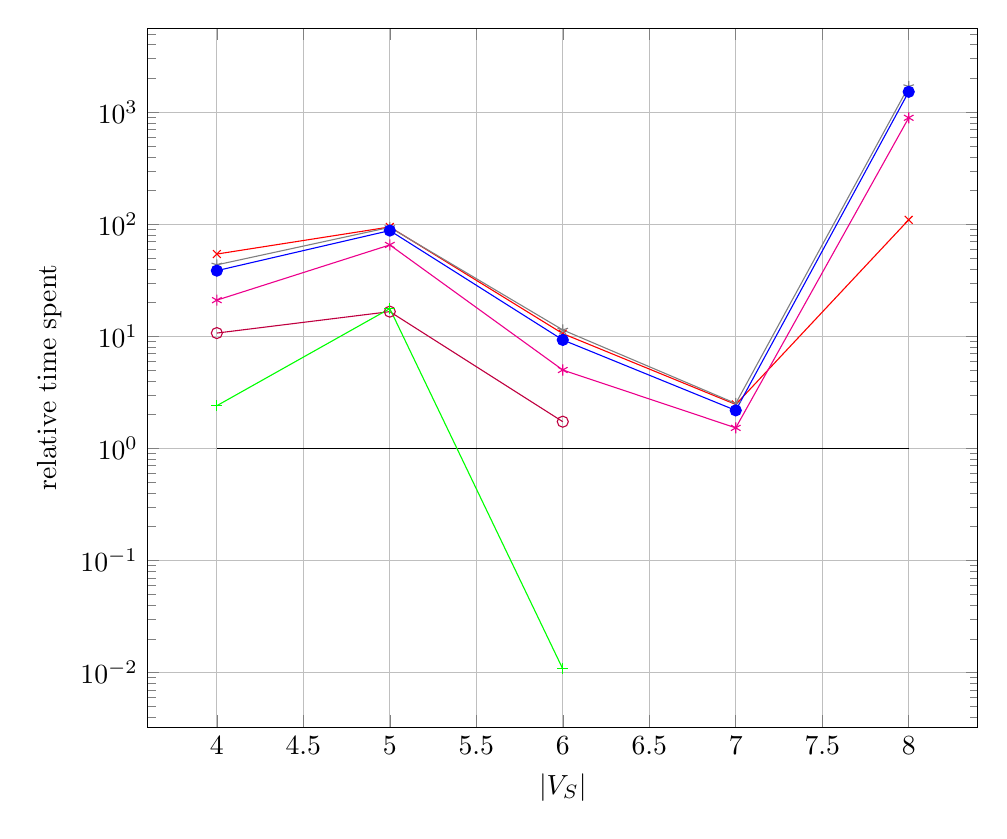
\begin{tikzpicture}
    \begin{axis}[
        xlabel=$|V_S|$,
        ylabel=relative time spent,
        ymode=log,
        legend style={at={(0.9,0.1)},anchor=south east},
        width=\textwidth,
		y tick label style={/pgf/number format/sci},
        ymajorgrids,
        xmajorgrids,		
    ]
\addplot [mark=none, black] plot coordinates {
        (4,1) (8, 1)};


%    \node[] at (axis cs: 9,1.1) {Awaiting test results (CAES server)};


\addplot[
        mark=x,
        red,
    ] plot coordinates {
        (4,54.244632157024924)
        (5,94.67410125160248)
        (6,10.579022919199833)
        (7,2.467884806621709)
        (8,109.61796961417762)
};
%    \addlegendentry{DFS}
\addplot[
        mark=o,
        purple,
    ] plot coordinates {
        (4,10.696848569213739)
        (5,16.61647755676102)
        (6,1.7322365504694384)
};
%    \addlegendentry{GDFS O IP}


\addplot[
        mark=star,
        gray,
    ] plot coordinates {
        (4,43.465930808198564)
        (5,93.92255198591933)
        (6,11.412954212374762)
        (7,2.518522472050785)
        (8,1697.6384316902834)
};
%    \addlegendentry{GDFS C}


\addplot[
        mark=*,
        blue,
    ] plot coordinates {
        (4,38.576420798557756)
        (5,87.89857301021381)
        (6,9.292817526299109)
        (7,2.183982399647286)
        (8,1521.5144724464335)
};
%    \addlegendentry{K-Path}


\addplot[
        mark=+,
        green,
    ] plot coordinates {
        (4,2.4051156279390042)
        (5,17.69226975418839)
        (6,0.01077006183520568)
};
%    \addlegendentry{CP}


\addplot[
        mark=asterisk,
        magenta,
    ] plot coordinates {
        (4,21.03540301694324)
        (5,65.43192659713577)
        (6,5.008411731723122)
        (7,1.525357905120218)
        (8,892.0214429471364)
};
%    \addlegendentry{GDFS A IP}


	
    \end{axis}
    \end{tikzpicture}
\caption{$|V_T|=5*|V_S|$ (no caching)}

\end{subfigure}
}
\resizebox{0.28\textheight}{!}{
\begin{subfigure} {0.5\linewidth}

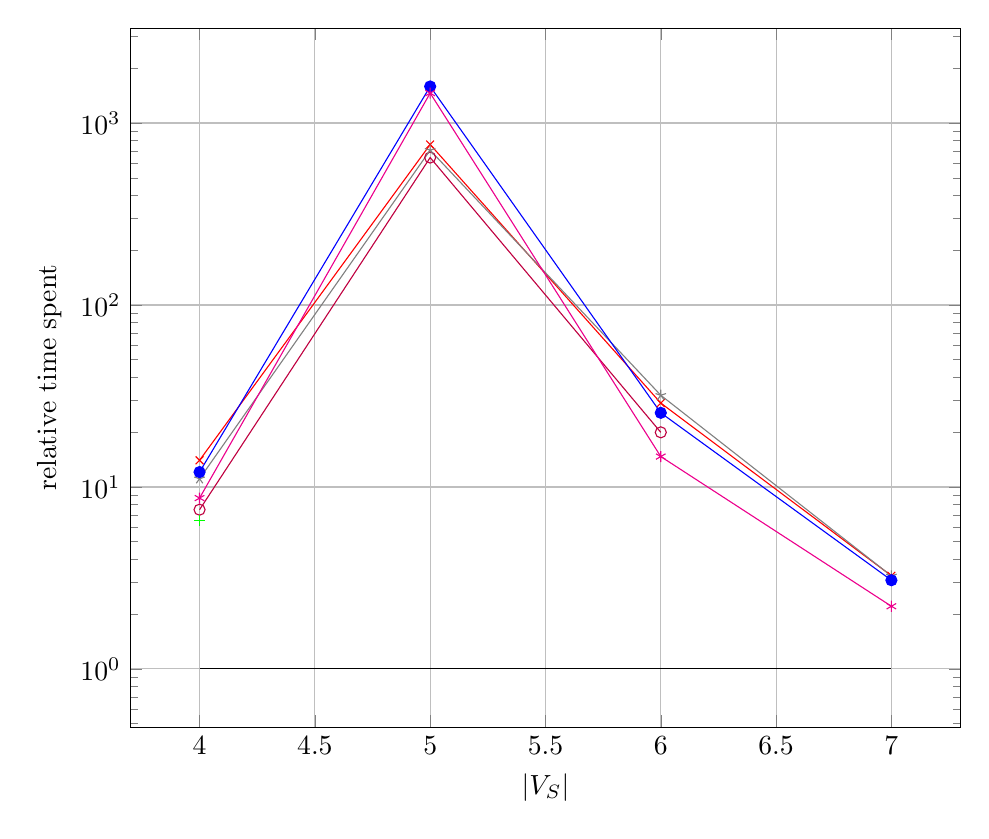
\begin{tikzpicture}
    \begin{axis}[
        xlabel=$|V_S|$,
        ylabel=relative time spent,
        ymode=log,
        legend style={at={(0.9,0.1)},anchor=south east},
        width=\textwidth,
		y tick label style={/pgf/number format/sci},
        ymajorgrids,
        xmajorgrids,		
    ]
\addplot [mark=none, black] plot coordinates {
        (4,1) (7, 1)};

%    \node[] at (axis cs: 9,1.1) {Awaiting test results (CAES server)};


\addplot[
        mark=x,
        red,
    ] plot coordinates {
        (4,14.014442936425434)
        (5,762.1422676420387)
        (6,28.909066998258137)
        (7,3.2500045042967773)
};
%    \addlegendentry{DFS}


\addplot[
        mark=o,
        purple,
    ] plot coordinates {
        (4,7.500984134455194)
        (5,645.9950612990576)
        (6,19.964026565489586)
};
%    \addlegendentry{GDFS O IP}


\addplot[
        mark=star,
        gray,
    ] plot coordinates {
        (4,11.095723351464535)
        (5,709.242281166574)
        (6,31.912378240077096)
        (7,3.2455637430524833)
};
%    \addlegendentry{GDFS C}


\addplot[
        mark=*,
        blue,
    ] plot coordinates {
        (4,12.071862186804472)
        (5,1588.441230780402)
        (6,25.547353262290816)
        (7,3.0715704037334586)
};
%    \addlegendentry{K-Path}
\addplot[
        mark=+,
        green,
    ] plot coordinates {
        (4,6.572698252534947)
};
%    \addlegendentry{CP}


\addplot[
        mark=asterisk,
        magenta,
    ] plot coordinates {
        (4,8.686387496374607)
        (5,1460.2833829253511)
        (6,14.692897155453814)
        (7,2.2099232478638378)
};
%    \addlegendentry{GDFS A IP}


	
    \end{axis}
    \end{tikzpicture}
\caption{$|V_T|=5*|V_S|$ (cached)}

\end{subfigure}
}

\caption{Performance of our algorithm with the distance based target graph vertex order relative to the performance of the algorithm with the degree-based target graph vertex order. ``refuse longer paths" and contraction are disabled and we use no pruning. Data points above the black reference line denote that this ordering introduces more delay, and data points below the reference line denote that this ordering saves time. Note the logarithmic y-axis.}		
\label{fig:DistanceVersusDegree}
\end{figure}

